\documentclass{article}
\usepackage{amsmath}
\usepackage{amssymb}
\usepackage{natbib}
\usepackage{textcomp}
\usepackage{graphicx}
\usepackage{ragged2e}
\usepackage{geometry}
\usepackage{tikz}
\usetikzlibrary{positioning}

\newgeometry{
    top = 2.5cm,
    lmargin = 4cm,
    rmargin = 3cm,
    bottom = 2.5cm
}

\title{
  \textbf{
    \huge Technical University of Munich \\ Campus Straubing \\ Faculty of Bioinformatics
        }\\
  \vspace{0,25cm}
  \huge Final report: Research internship \\ Applying Deep Reinforcement Learning to \textit{Lunar Lander}
  }
\author{\huge Krystian Budkiewicz}
\date{\huge 01.12.2022}

\begin{document}
\maketitle
\vspace{4cm}
\tableofcontents
\pagebreak

\begin{centering}
    \section*{Abstract}
    This document summarizes my 6-week research internship under assistance of PhD student Jonathan Pirnay at the Faculty of Bioinformatics led by Prof. Dominik Grimm at TUM Campus Straubing, during which I implemented a Deep Q-Algorithm solving \textit{Lunar Lander} environment. The influence of learning rate and start, end and termination variables of linear epsilon-decay on score gained by the agent in the environment, as well as loss-function during the runs were examined.
\end{centering}

\section{Introduction}
In the past decade great progress has been made in the subject of machine learning (ML). One of the most influential steps, has been the usage of neural networks in a subset of ML, reinforcement learning (RL), known as deep reinforcement learning (deep RL), achieving or in some cases outperforming human level performance \cite{mnih2015human}. Since then, the usage of deep RL exploded and has become state of the art method for solving complex problems in multiple areas such as playing video games \cite{mnih2015human}\cite{mnih2013playing}, board games \cite{silver2016mastering}\cite{silver2018general} or optimizing mathematical calculations \cite{fawzi2022discovering}. An advantage of deep RL over rule-based algorithms is their robustness and ability to solve a plethora of different problems with similar approach, rather than being confined to one task, for which the rules have to be explicitly written.

During my internship, I was introduced to the basic ideas of RL and deep learning under the assistance of PhD student Jonathan Pirnay. Using knowledge gained in both of these topics, I programmed a Deep-Q-Algorithm solving a benchmark toy problem of \textit{Lunar Lander}. This document gives a short introduction to RL, \textit{Lunar Lander} suite and deep Q-learning, and  presents results of my inquiries to variables of the algorithm, as well as their influence on the agent.

\section{Reinforcement Learning}
Reinforcement learning (RL) is a subset of machine learning (ML), which is concerned with usage of big data-sets for training an artificial intelligence  (AI) agent in order to optimize its behaviour \cite{lapan2018deep}. Given a set of states $\mathcal{S}$, actions $\mathcal{A}$ and rewards $\mathcal{R}$, an agent interacts with an environment based on a policy $\pi$ depending on current state $s\in\mathcal{S}$ and possible actions $a\in\mathcal{A}$ that can be taken from that state (Eq. \ref{eqn:policy}), in order to get rewards $r\in\mathcal{R}$, in a process known as a Markov decision process (MDP); the main dogma being, that every interaction between an agent and an environment can be modeled as maximisation of reward received by an agent after an interaction with its surroundings, by choosing an optimal its policy $\pi^{*}$.

\begin{equation}
    \label{eqn:policy}
    \pi(s|a)=\mathbb{P}[A_t=a|S_t=s]
\end{equation}

Because of numerous variables influencing how much reward an agents gets, the only significant outcome is the amount of reward gained and value of the next state-action pair $(s',a')$ after the interaction - a target $G_t$. Given a state-action pair $(s,a)$ one can determine the value $Q^\pi$ of the whole interaction, i.e. reward $r$ and next state-action pair $(s',a')$, via Bellman equation (Eq. \ref{eqn:bellman}).

\begin{equation}
\label{eqn:bellman}
Q^\pi(s,a) = r+\gamma \max_{a'}Q^\pi(s',\pi(a'))
\end{equation}
\\
TXT.

\newpage
\section{Lunar Lander}
The game of \textit{Lunar Lander} is a \textit{Box2D} environment from OpenAI \textit{Gym} library, based on a game with the same name for a famous 70s game console Atari 2600, used as a benchmark for DQN-Algorithms \cite{brockman2016openai}. The task of the game is to land a lunar lander onto a designated area in the middle of the screen without crashing the vehicle or leaving the bounds of the environment (Figure \ref{fig:lunarlander}.). Each episode starts with randomised state-vector $s$ with 8 variables (such as x position, y position, angle, velocity, etc.) restricted to a specific, discrete range of values for each variable. Based on its current state $s$, the agent can evaluate its position and interact with the environment through 4 actions: (a) doing nothing or (b, c, d) turning one of the three engines on or off (either left, right or bottom). For every action $a$ chosen by the agent, the environment makes a step (corresponding to a frame within the game) calculating the next state $s'$ and rewarding the agent with reward $r$, depending on the action taken and new state $s'$ within the environment. This cycle of evaluating starts all over again, until the episode gets terminated - either due to crashing or turning over the lander, leaving the bounds of the environment, running out of time(steps) or successfully landing in the designated area. After each termination, a new episode with randomised starting position (state $s$) gets initiated, until the run is over.

The environment is considered solved when the moving average score achieved by the agent in last 100 episodes equals or is greater than 200.\\

\begin{figure}[h]
    \centering
    \includegraphics[width=0.8\linewidth]{figs/lunarlander.jpg}
    \caption{A screenshot of the environment. Lunar lander (violet) descending towards the moon surface (white) onto the designated area between the flags.}
    \label{fig:lunarlander}
\end{figure}

% \pagebreak
\section{Deep Q-Learning}
Deep Q-Learning combines the usage of action-state function $Q^\pi$ with neural networks. A neural network (Figure \ref{fig:nn}.), which can be thought of as a function approximator, consists of neurons combined in a complex network with multiple layers, which process the input data (state $s$ of the agent) and outputs an evaluation ($Q^{\pi}$-values for every action $a$ an agent can take).

A neural network can be described with a matrix of weights $\textbf{w}$ connecting each neuron in the network. For every step the agent takes, the input gets processed through a local network (current evaluation of the state) and target network (estimation of what the agent thinks is a correct evaluation of the environment). Squared difference between these two networks equal a loss $\mathcal{L}$ - a measure how good the current model is.

\begin{equation}
    \label{eqn:loss}
    \mathcal{L} = \alpha(r+\gamma\max_{s,a} Q(s',a')-Q(s,a))^2
\end{equation}
\\
Based on the value of $\mathcal{L}$, weights of the local network get adjusted towards descending gradient within the action-value space using chain rule in such a way, as to minimise $\mathcal{L}$ in the next evaluation - a process called backpropagation (Eq. \ref{eqn:grad}). After multiple steps and episodes during the run, each weight in the matrix $\textbf{w}$ gets set to such a value allowing the agent to optimally decide the course of action.

\begin{equation}
    \label{eqn:grad}
    \Delta\textbf{w}=-\frac{1}{2}\alpha\nabla_{w}J(\textbf{w})
\end{equation}

\begin{figure}[ht]
    \centering
    \label{fig:nn}
    \vspace{0.5cm}
    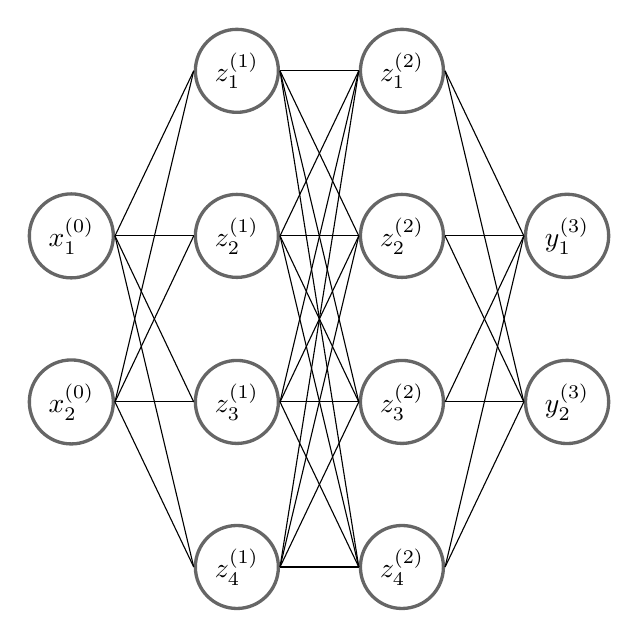
\begin{tikzpicture}[roundnode/.style={circle, draw=black!60, very thick, minimum size=8mm}]
    %Nodes
    \node[roundnode]        (in0)                          {$x_1^{(0)}$};
    \node[roundnode]        (in1)           [below=of in0] {$x_2^{(0)}$};
    \node[roundnode]        (h1)            [right=of in0] {$z_2^{(1)}$};
    \node[roundnode]        (h0)            [above=of h1] {$z_1^{(1)}$};
    \node[roundnode]        (h2)            [right=of  in1] {$z_3^{(1)}$};
    \node[roundnode]        (h3)            [below=of  h2] {$z_4^{(1)}$};
    \node[roundnode]        (g1)            [right=of h1] {$z_2^{(2)}$};
    \node[roundnode]        (g0)            [right=of h0] {$z_1^{(2)}$};
    \node[roundnode]        (g2)            [right=of  h2] {$z_3^{(2)}$};
    \node[roundnode]        (g3)            [right=of  h3] {$z_4^{(2)}$};
    \node[roundnode]        (o0)            [right=of  g1] {$y_1^{(3)}$};
    \node[roundnode]        (o1)            [right=of  g2] {$y_2^{(3)}$};

    %Lines
    \draw (in0.east) -- (h0.west);
    \draw (in0.east) -- (h1.west);
    \draw (in0.east) -- (h2.west);
    \draw (in0.east) -- (h3.west);
    \draw (in1.east) -- (h0.west);
    \draw (in1.east) -- (h1.west);
    \draw (in1.east) -- (h2.west);
    \draw (in1.east) -- (h3.west);
    \draw (h0.east) -- (g0.west);
    \draw (h0.east) -- (g1.west);
    \draw (h0.east) -- (g2.west);
    \draw (h0.east) -- (g3.west);
    \draw (h1.east) -- (g0.west);
    \draw (h1.east) -- (g1.west);
    \draw (h1.east) -- (g2.west);
    \draw (h1.east) -- (g3.west);
    \draw (h2.east) -- (g0.west);
    \draw (h2.east) -- (g1.west);
    \draw (h2.east) -- (g2.west);
    \draw (h2.east) -- (g3.west);
    \draw (h3.east) -- (g0.west);
    \draw (h3.east) -- (g1.west);
    \draw (h3.east) -- (g2.west);
    \draw (h3.east) -- (g3.west);
    \draw (g0.east) -- (o0.west);
    \draw (g0.east) -- (o1.west);
    \draw (g1.east) -- (o0.west);
    \draw (g1.east) -- (o1.west);
    \draw (g2.east) -- (o0.west);
    \draw (g2.east) -- (o1.west);
    \draw (g3.east) -- (o0.west);
    \draw (g3.east) -- (o1.west);
    \end{tikzpicture}
    \caption{An exemplary neural network with 2 inputs, 2 hidden layers consisting of 4 neurons each and 2 outputs.}
\end{figure}

Additionaly, in order to decorrelate the experiences of the agent and further speed up the learning process, replay memory - a container storing past experiences - can be implemented \cite{liu2018effects}. Every time a step is made, the agent compares their policy through the local neural network with past policy through target neural network, calculating the loss $\mathcal{L}$.

\begin{equation}
    \mathcal{L} = \frac{1}{N}\sum^{N}_{i=1}{(Q_{local}-Q_{target})^2}
\end{equation}

\section{Training procedure}
In the beginning, parameters set during each run were based on parameters found in code online \footnotemark. After unsuccessful runs these parameters were randomly changed in order to improve agents behaviour, until the agent could solve the environment in 5 subsequent runs. Parameters used during these runs are tablified in Table \ref{table:standard}. and will be later referred to as "standard parameters". Once 5 successful runs were achieved, one of the parameters was changed and its influence on the score achieved by the agent and loss during next 5 runs was noted. Optimization of the neural networks was done using Adam algorithm \cite{kingma2014adam}.

\begin{table}[ht]
    \caption{Parameters used resulting in first successful runs. Referred to as "standard parameters".}
    \vspace{0.5cm}
    \label{table:standard}
    \centering
    \begin{tabular}{cc}
        \hline
        \textbf{Parameter}                      & \textbf{Value} \\
        \hline
        Maximum amount of episodes              & 1500      \\
        Maximum amount of steps                 & 1000      \\
        Batch size                              & 100       \\
        Replay memory size                      & 100000    \\
        Amount of hidden layers                 & 3         \\
        Amount of neurons per hidden layer      & 64        \\
        Target network update frequency         & 6         \\
        Network parameter update factor $\tau$  & 2.5e-3    \\
        Learning rate $\alpha$                  & 2.5e-4    \\
        Discount factor $\gamma$                & 0.99      \\
        $\varepsilon$-start                     & 1         \\
        $\varepsilon$-end                       & 0.01      \\
        $\varepsilon$-term                      & 1000      \\
        \hline
    \end{tabular}
\end{table}

\footnotetext{https://goodboychan.github.io/python/reinforcement_learning/pytorch/udacity/2021/05/07/DQN-LunarLander.html\#Training-Process}

\newpage
\section{Results and Discussion}

\subsection*{Behaviours of the agent during training}
In order to solve the environment and maximize the reward from given episode the agent tried multiple tactics: (a) hovering with the lunar lander directly or high above the landing area, then slowly descending onto the designated area, (b) dropping fast towards the ground while not breaking the lander, then using one of the engines on the side to push the lander towards the landing area and (c) the most resembling human-like play-style, slowing down from the initial state and descending in a swing-like motion towards the landing area.

During multiple training cycles the agent showed similar behaviours, which resulted in achieving lower scores, such as not slowing down enough from the starting condition and crashing the lander into the ground, flipping the lander over, not solving the environment in given time (steps), not turning the engines off while on the landing platform or getting out of environments bounds, thus either terminating the episode (in the case of crashing and flipping over) or achieving a huge negative score.

\subsection*{Linear $\varepsilon$-decay}

\subsubsection*{$\varepsilon$-start}
$\varepsilon$-start is the value of $\varepsilon$ with which the first state gets initialized.

Smaller $\varepsilon$-start lead to smaller probability of taking a random action by the agent, thus increasing the mean score, starting exploitation phase and solving the environment earlier - $\varepsilon$-start = 0.7 being the best value found (Figure \ref{fig:start}.). Also, smaller $\varepsilon$-start tend to minimise the loss-function across the episode faster than values closer to 1 (Figure \ref{fig:start_loss}.), due to smaller slope of $\varepsilon$-decay.

\subsubsection*{$\varepsilon$-end}
$\varepsilon$-end is the value of $\varepsilon$ which remains constant  until the termination of the run after episode defined by $\varepsilon$-term has been achieved.

Small $\varepsilon$-end lead to faster increase of score during the latter part of the episode (Figure \ref{fig:end}.). After termination of $\varepsilon$, smaller $\varepsilon$-end tend to start exploitation phase faster, thus leading to a plateau in score. Increasing $\varepsilon$-end to an optimum leads to faster solving of the environment by the agent - $\varepsilon$-end = 0.05 being the best value found.

\subsubsection*{$\varepsilon$-term}
Termination of $\varepsilon$ at episode $e$, is the episode $e$ at which $\varepsilon$-end is reached.

Bigger $\varepsilon$-term increase the time-duration of exploration phase of the agent and lead to later increase of score in latter parts of the episode - $\varepsilon$-term = 1200 being the best value found (Figure \ref{fig:term}.). Because $\varepsilon$-term sets at which episode $\varepsilon$-end is reached, it also sets the steepness of the $\varepsilon$-decay and defines when exploitation phase starts, thus shifting the "take-off" of the score during the episode, with bigger values allowing for longer exploration of the environment.

% \begin{figure}[ht]
%     \caption{Scores test with variable $\varepsilon$-end (a), Scores test with variable $\varepsilon$-start (b) and Scores test with variable $\varepsilon$-term (c)}
%     \centering
%     \begin{subfigure}
%         \centering
%         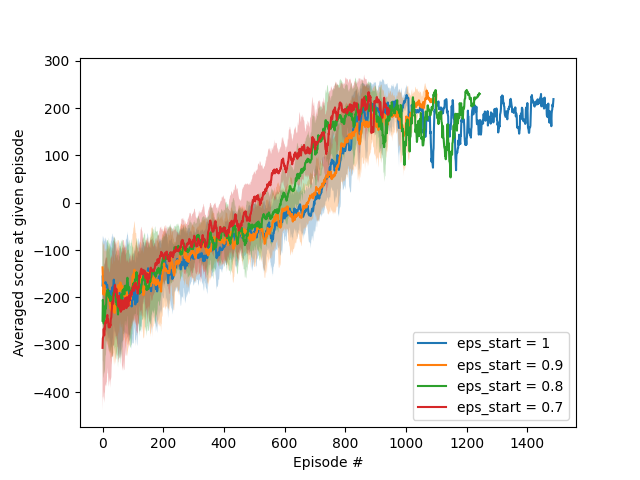
\includegraphics[width=0.333\linewidth]{figs/EPS_START.png}
%     \end{subfigure}
%     \begin{subfigure}
%         \centering
%         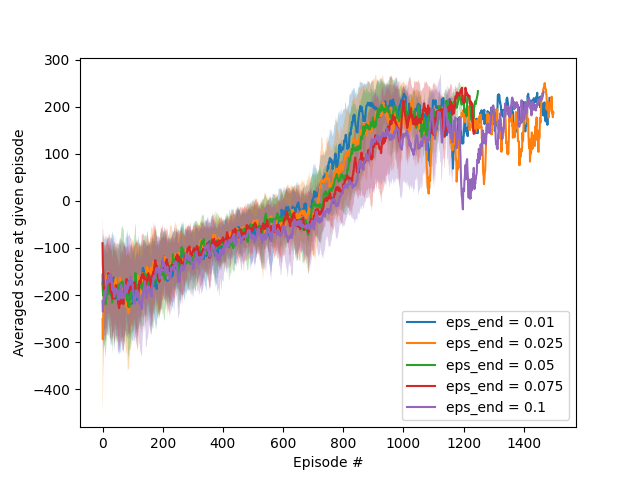
\includegraphics[width=0.333\linewidth]{figs/EPS_END.png}
%     \end{subfigure}
%     \begin{subfigure}
%         \centering
%         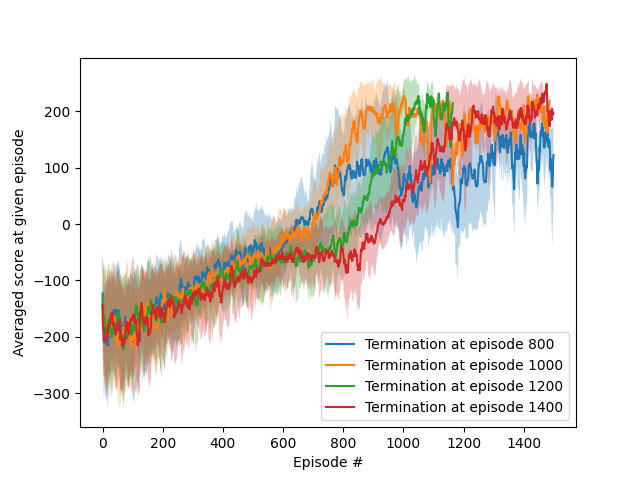
\includegraphics[width=0.333\linewidth]{figs/EPS_TERM.png}
%     \end{subfigure}
%     \label{fig:scores}
% \end{figure}

\subsection*{Learning rate}
Decreasing the value of $\alpha$ increased the amount of episodes needed to solve the environment - $\alpha = 5e-4$ being the best value found (Figure \ref{fig:lr}.). Smaller learning rates, combined with fast $\varepsilon$-decay and small $\varepsilon$-end, disallow the agent to explore new possibilities within the environment after $\varepsilon$-end is reached. Because of that, the agent sticks with the best policy learned up to $\varepsilon$-term, resulting in stagnation of score further in the run, with only occasional variations. Slower $\varepsilon$-decay could yield better results by allowing the agent to explore for longer. Also, smaller learning rates increase average loss during the episode (Figure \ref{fig:lr_loss}.).

\newpage
\addcontentsline{toc}{section}{Methods}
\section*{Methods}
Deep Q-Algorithm was written in \textit{Python} (v. 3.9) with \textit{PyTorch} (v. 1.12.1) and \textit{NumPy} (v. 1.23.3) libraries, as well as certain functions from \textit{collections} library. The \textit{Lunar Lander} environment was imported from \textit{Gym} (v. 0.26.1) library. The code is available on GitHub (https://github.com/kbudkiewicz/research-internship-RL).

Scores and loss-function were averaged across the whole set of these 5 runs for each change in parameter. Standard deviation $\sigma$ was calculated at each episode. Both score average and standard deviation were plotted in a linear plot with shaded area error-bars using moving average of last 10 values (average score or loss) and standard deviations (shaded area). Plots were written with \textit{Matplotlib} library in \textit{Python}.

\addcontentsline{toc}{section}{List of figures}
\section*{List of Figures}

\begin{figure}[ht]
    \centering
    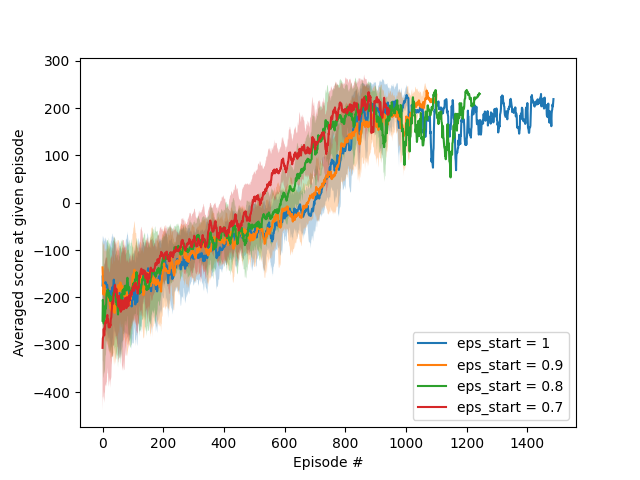
\includegraphics[width=0.8\linewidth]{figs/EPS_START.png}
    \caption{Influence of $\varepsilon$-start on score gained by the agent during the episode. All other parameters remaining standard.}
    \label{fig:start}
\end{figure}

\begin{figure}
    \centering
    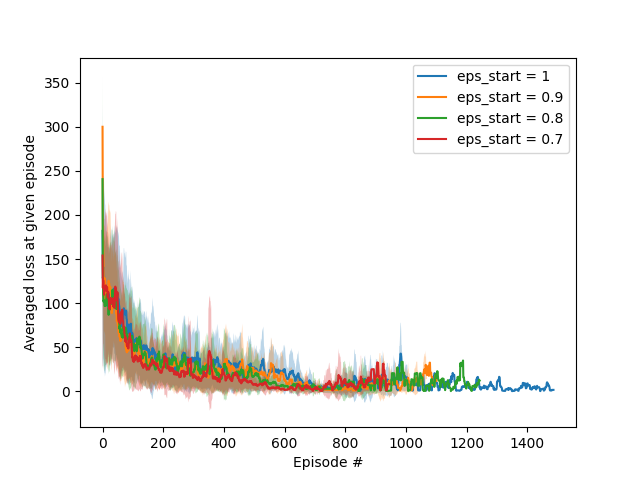
\includegraphics[width=0.8\linewidth]{figs/EPS_START(loss).png}
    \caption{Influence of $\varepsilon$-start on score gained by the agent during the episode. All other parameters remaining standard.}
    \label{fig:start_loss}
\end{figure}

\begin{figure}
    \centering
    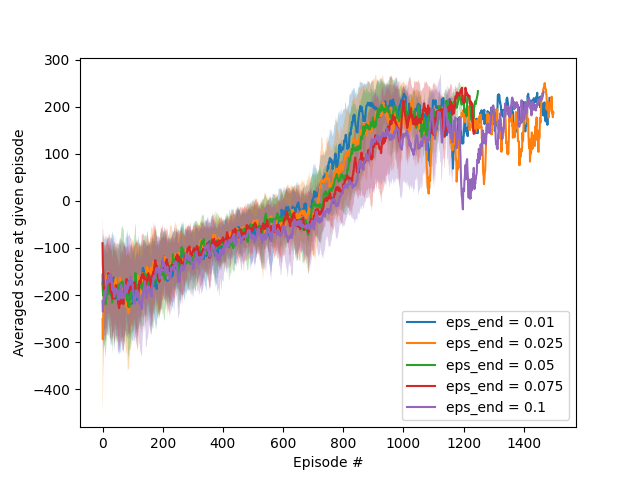
\includegraphics[width=0.8\linewidth]{figs/EPS_END.png}
    \caption{Influence of $\varepsilon$-end on score gained by the agent during the episode. All other parameters remaining standard.}
    \label{fig:end}
\end{figure}

\begin{figure}
    \centering
    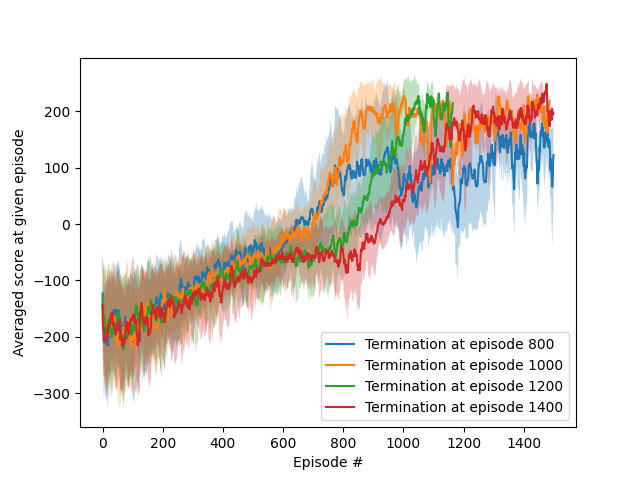
\includegraphics[width=0.8\linewidth]{figs/EPS_TERM.png}
    \caption{Influence of $\varepsilon$-term on score gained by the agent during the episode. All other parameters remaining standard.}
    \label{fig:term}
\end{figure}

\begin{figure}
    \centering
    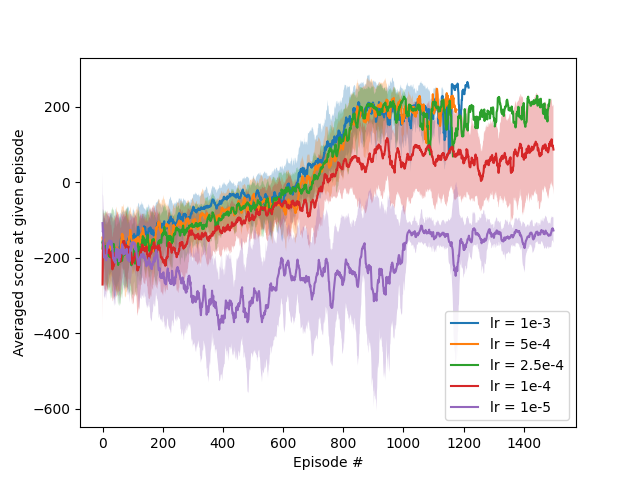
\includegraphics[width=0.8\linewidth]{figs/LR.png}
    \caption{Averaged scores with varied learning rate $\alpha$. All other parameters remaining standard.}
    \label{fig:lr}
\end{figure}

\begin{figure}
    \centering
    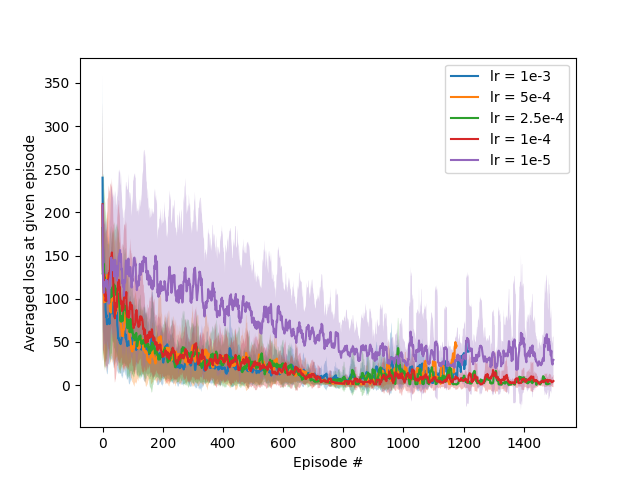
\includegraphics[width=0.8\linewidth]{figs/LR(loss).png}
    \caption{Averaged scores with varied learning rate $\alpha$. All other parameters remaining standard.}
    \label{fig:lr_loss}
\end{figure}

\newpage
\addcontentsline{toc}{section}{References}
\bibliographystyle{plain}
\bibliography{refs}

\end{document}